\documentclass{beamer}

\usetheme{default} 
\usepackage{graphicx}
\usepackage{amsmath}
\usepackage{amssymb}
\usepackage{mathtools}
\usepackage{hyperref}
\hypersetup{
    colorlinks=true,
    linkcolor=blue,
    filecolor=magenta,      
    urlcolor=blue
}

\newcommand{\R}{\mathbb{R}}
\newcommand{\Z}{\mathbb{Z}}
\newcommand{\norm}[1]{\left\lVert#1\right\rVert}


\title{Group Equivariant Convolutional Networks}
\author{Daniel Ralston}
\date{1/22/2024}

\begin{document}

% Title Slide
\begin{frame}
  \titlepage
\end{frame}

%It seems as though these networks aren't used as much now, why is this?

% Table of Contents
\begin{frame}{Agenda}
    \begin{itemize}
        \item Introduction and Motivation
        \item Related Works
        \item Background: Groups, Group Actions, and Equivariance
        \item Methods: $G$ Equivariant Convolution
        \item Results
        \item Demonstration of the Code
        \item Conclusion
    \end{itemize}
\end{frame}

% Introduction
\section{Introduction}
\begin{frame}{Introduction}
    \begin{itemize}
        \item $G$-CNNs extend traditional CNNs by exploiting symmetries in the feature space, increasing model efficiency and robustness.
        \item Introduced to improve parameter efficiency and reduce computational complexity while maintaining performance.
        \item Group convolutions factorize convolutions based on group theory, enabling weight sharing across different transformations.
        \item Key for advancing deep learning in scenarios with limited data, improving generalization across transformed inputs.
        \item Pioneered new approaches to invariant and equivariant feature learning, laying foundations for subsequent architectural innovations.
    \end{itemize}
\end{frame}

% Related Works
\section{Related Works}
\begin{frame}{Related Works}
    \begin{itemize}
        \item Invariant representations improve image analysis, achieved by pose normalization and group averaging (Lowe, 2004; Reisert, 2008; Kondor, 2007) and extended by scattering convolution networks (Bruna and Mallat, 2013).
        \item Scattering networks, which use wavelet convolutions and nonlinearities, have been adapted for stable invariants in object and texture recognition (Sifre and Mallat, 2013; Oyallon and Mallat, 2015).
        \item Equivariant representations have been advanced through architectures like transforming autoencoders (Hinton et al., 2011) and convolutional architectures (Gens and Domingos, 2014) with unconventional learning applications (Agrawal et al., 2015).
        \item High-dimensional transformations and symmetry exploitation in convolutional networks have been utilized for tasks like galaxy morphology prediction, enhancing vision-related models (Dieleman et al., 2015; 2016; Cohen and Welling, 2014; 2015).
      \end{itemize}
\end{frame}

% Background
\section{Background}
\begin{frame}{Groups}
    \begin{itemize}
        \item A \emph{group} is a set $G$ with a binary operation $\cdot$ such that:
        \begin{enumerate}
            \item $G$ is closed under $\cdot$
            \item $\cdot$ is associative
            \item There exists an identity element $e \in G$ such that $e \cdot g = g \cdot e = g$ for all $g \in G$
            \item For each $g \in G$, there exists an inverse $g^{-1} \in G$ such that $g \cdot g^{-1} = g^{-1} \cdot g = e$
        \end{enumerate}
        \item In this paper, the authors focus on groups of rigid transformations of the plane (e.g. subgroups of $SE(2)$, the 2-dimensional special Euclidean group)
    \end{itemize}
\end{frame}

\begin{frame}{$p4$ and $p4m$}
    \begin{itemize}
        \item $p4$ -- all 2-dimensional integer translations and rotations by multiples of $\frac{\pi}{2}$
        \begin{itemize}
            \item The underlying set can be described as a set of matrices where $r \in \{0, 1, 2, 3\}$ and $u, v \in \mathbb{Z}$
            $$g(r, u, v) = \begin{bmatrix}
                \cos(\frac{\pi}{2}r) & -\sin(\frac{\pi}{2}r) & u \\
                \sin(\frac{\pi}{2}r) & \cos(\frac{\pi}{2}r) & v \\
                0 & 0 & 1
            \end{bmatrix}$$
        \end{itemize}
        \item $p4m$ -- all 2-dimensional integer translations, rotations by multiples of $\frac{\pi}{2}$, and mirror reflections
        \begin{itemize}
            \item For $r \in \{0, 1, 2, 3\}$, $u, v \in \mathbb{Z}$, and $m \in \{0, 1\}$
            $$g(m, r, u, v) = \begin{bmatrix}
                (-1)^m\cos(\frac{\pi}{2}r) & (-1)^{m+1}\sin(\frac{\pi}{2}r) & u \\
                \sin(\frac{\pi}{2}r) & \cos(\frac{\pi}{2}r) & v \\
                0 & 0 & 1
            \end{bmatrix}$$
        \end{itemize}
        \item In both cases, the binary operation is matrix multiplication
    \end{itemize}
\end{frame}

\begin{frame}{Group Actions}
    %mention how a group (R, +) acts on a vector space by scalar multiplication
    \begin{itemize}
        \item Critical to this paper, the authors use the fact that these groups act on the set of images.
        \item A group $G$ is said to act on a set $X$ if there exists a function $\gamma: G\times X \to X$ such that 
        $$\gamma(e, x) = x \text{ ($e$ is the identity element of $G$)}$$
        $$\gamma(g_1, \gamma(g_2, x)) = \gamma(g_1g_2, x)$$
        \item $p4$ and $p4m$ act on $\Z^2$ (specifically $\Z^2 \times \{1\} \subset \R^3$) by matrix-vector multiplication:
        \begin{itemize}
            \item Ex: For $A\in p4$ and $[u, v, 1]^T \in \Z^2 \times \{1\}$, $$A[u, v, 1]^T = [u', v', 1]^T \in \Z^2 \times \{1\}$$
        \end{itemize} 
    \end{itemize}
\end{frame}

\begin{frame}{Acting on the set of images}
    \begin{itemize}
        \item The authors describe the set of images as the collection of functions $f: \Z^2 \to \R^K$ (where $f$ has compact (rectangular) support)
        \item $p4$ and $p4m$ act on the the set of images $\{f\}$ with the function $L$:
        $$L_g(f)(x) = f(g^{-1}x)$$
        where $g^{-1}x$ denotes matrix-vector multiplication
    \end{itemize}
\end{frame}

\begin{frame}{Equivariance}
    \begin{itemize}
        \item Let $G$ be a group acting on $X$ and $Y$.  A function $f:X \to Y$ is called \emph{equivariant} if 
        $$f(gx) = gf(x) \text{ for all $g$ in $G$ and $x$ in $X$}$$
        \item Fix a kernel $\Psi$ and denote $*$ as the convolution operator.  Suppose $G$ is the group of integer translations acting by $T$ on the set of images. 
         $$T(g,f)(x)= f(-g + x)$$ 
        \item For any image $f\in \{f\}$, the convolution operator $(\cdot)*\Psi: \{f\} \to \{f\}$ is equivariant with respect to translation:
        $$ (T(g, f) * \Psi)(x) = T(g, (f * \Psi))(x)$$
        (i.e. you can translate an image and then convolve it or you can first convolve the image and then translate the output)
    \end{itemize}
\end{frame}

\begin{frame}{Translation Equivariance}
    \begin{figure}
        \centering
        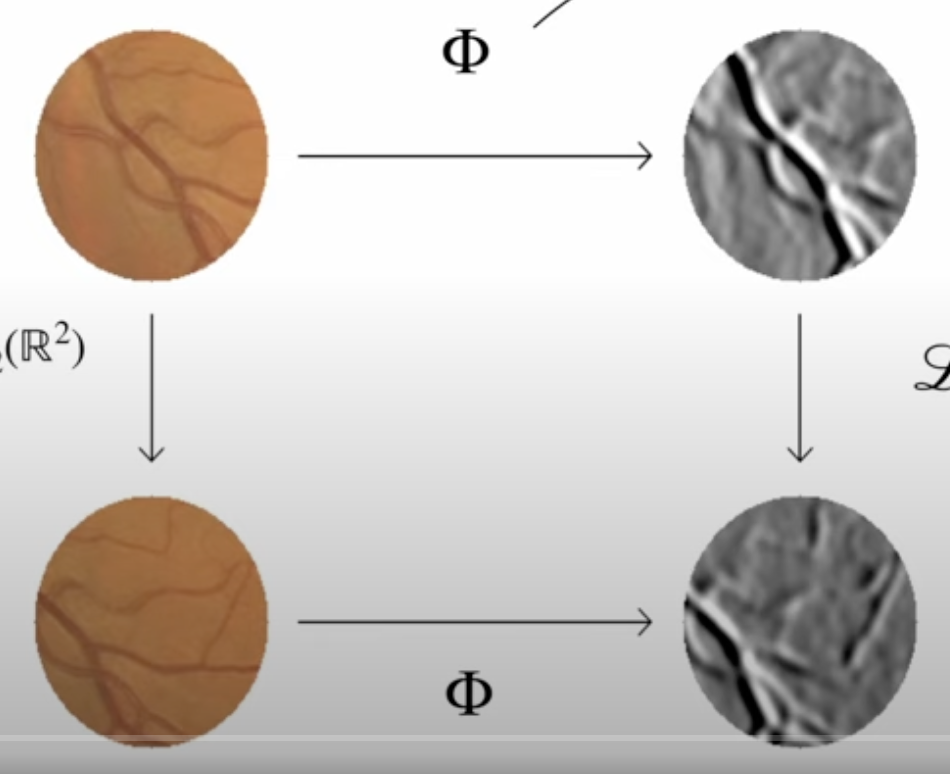
\includegraphics[width=0.5\textwidth, height=0.5\textheight]{Screenshot 2024-01-13 at 11.31.21 AM.png}
    \end{figure}
\end{frame}

\begin{frame}{Key Idea}
    \begin{itemize}
        \item The authors want a convolution operator that is equivariant with respect to the group action of $p4$ or $p4m$
        \item We want a convolution where inputting a rotated image is the same as inputting a non-rotated image, convolving, and then rotating the output
    \end{itemize}
\end{frame}

\section{Methods}

\begin{frame}{Group Equivariant Convolution}
    \begin{itemize}
        \item Let $f: \Z^2 \to \R^K$ be an image.  
        \item Let $G$ be either $p4$ or $p4m$ and let $\Psi$ be a kernel.  Then the \emph{group equivariant convolution} $*_G$ is defined as 
        $$[f *_G \Psi](g) = \sum_{y \in \Z^2}\sum_{k \in \{1, \dots, K\}} f_k(y)\Psi_k(g^{-1}y)$$
        $$\left(= \sum_{y \in \Z^2}\sum_{k \in \{1, \dots, K\}} f_k(gy)\Psi_k(y)\right)$$
    \end{itemize}
\end{frame}

\begin{frame}{Group Equivariant Convolution}
    \begin{itemize}
        \item Equivariance property -- denoting $L_g$ be the action of $g\in G$ on the set of images, 
        $$L_h(f *_G \Psi)(g) = L_h\left(\sum_{y \in \Z^2}\sum_{k \in \{1, \dots, K\}} f_k(y)\Psi_k(g^{-1}y)\right)$$
        $$= \sum_{y \in \Z^2}\sum_{k \in \{1, \dots, K\}} f_k(hy)\Psi_k(g^{-1}y)$$
        $$ = [L_h(f) *_G \Psi](g) \qquad \text{(note equivariance)}$$
        $$= \sum_{y \in \Z^2}\sum_{k \in \{1, \dots, K\}} f_k(y)\Psi_k(h^{-1}g^{-1}y) \text{ }$$
        $$= [f *_G L_{h^{-1}}(\Psi)](g)$$
    \end{itemize}
\end{frame}

\begin{frame}{A Subtlety}
    \begin{itemize}
        \item After the first layer of a $*_G$ convolution on an image $f$:
         $$[f *_G \Psi](g) $$
         letting $g$ vary, our output is a set of images $\{[f *_G \Psi](g)\}_{g\in G}$ that now also depends on $G$
         \item Thus, our filter needs to take elements of $G$ (translations, rotations, reflections) as inputs
    \end{itemize}
\end{frame}

\begin{frame}{Inner G-CNN Convolutions}
    \begin{itemize}
        \item For inner layers the convolutional operator $*_G$ is defined as 
        $$[f *_G \Psi](g) = \sum_{h \in G} \sum_{k \in \{1, \dots, K\}} f_k(h)\Psi_k(g^{-1}h)$$
        \item Equivariance property follows similarly as before:
        $$L_{u}([f *_G \Psi])(g) = L_{u}\left(\sum_{h \in G} \sum_{k \in \{1, \dots, K\}} f_k(h)\Psi_k(g^{-1}h)\right)$$
        $$= \sum_{h \in G} \sum_{k \in \{1, \dots, K\}} f_k(uh)\Psi_k(g^{-1}h)$$
        $$ = [L_{u}(f) *_G \Psi](g) $$
        $$ = [f *_G L_{u^{-1}}(\Psi)](g)$$
    \end{itemize}
\end{frame}

\begin{frame}{$G$-CNN Visualization}
    \begin{figure}
        \centering
        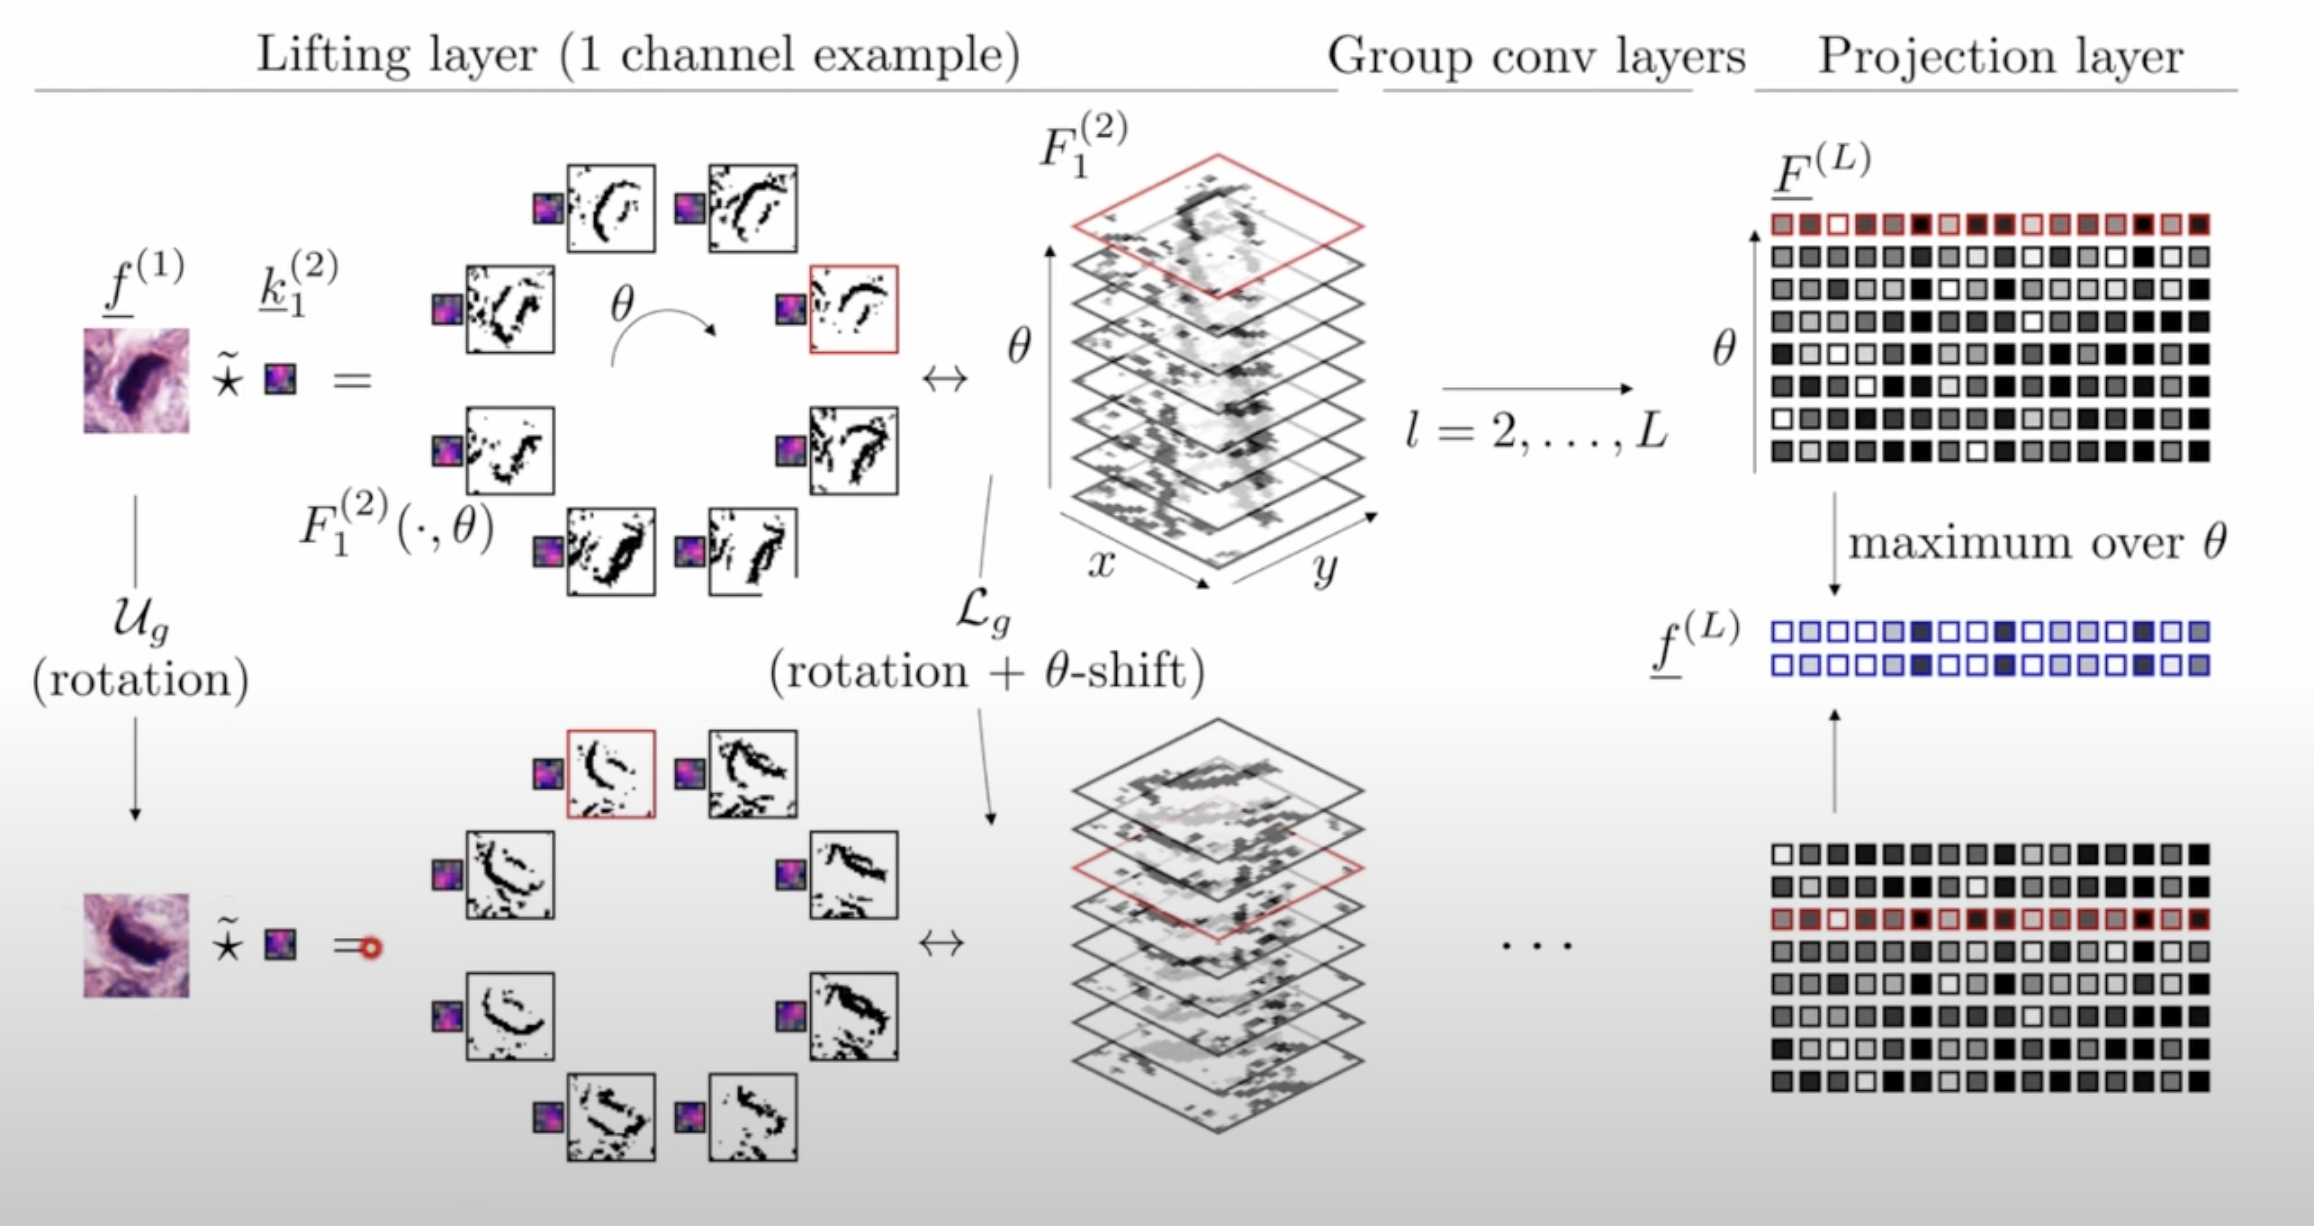
\includegraphics[width=\textwidth,height=\textheight,keepaspectratio]{Screenshot 2024-01-15 at 12.20.40 PM.png}
    \end{figure}
\end{frame}

\begin{frame}{Feature Maps}
    \begin{minipage}{0.5\textwidth}
        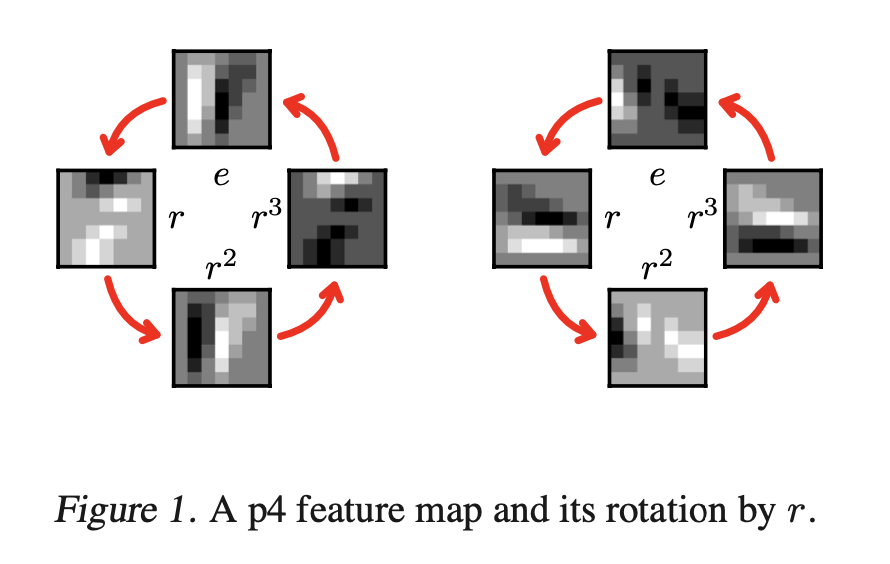
\includegraphics[width=\linewidth]{Screenshot 2024-01-13 at 11.28.41 AM.png} % replace with your first image file
        % \caption{Caption for image1}
    \end{minipage}%
    \begin{minipage}{0.5\textwidth}
        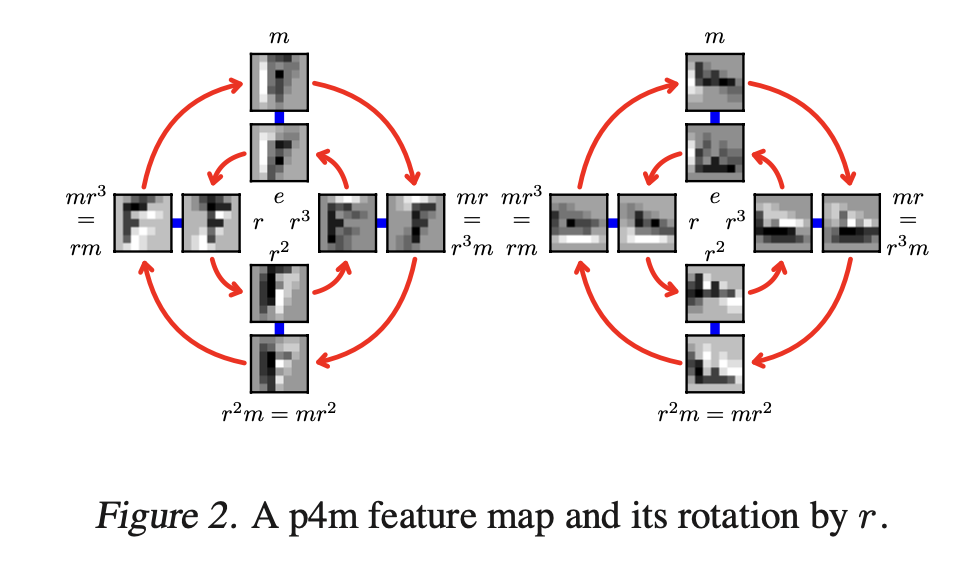
\includegraphics[width=\linewidth]{Screenshot 2024-01-13 at 11.28.51 AM.png} % replace with your second image file
        % \caption{Caption for image2}
    \end{minipage}
\end{frame}

\begin{frame}{Activations and Pooling}
    \begin{itemize}
        \item Activations commute with the group action $L$ on $\{f\}$: 
        $$L_g(\sigma(f(x))) = \sigma(f(g^{-1}x)) = \sigma(L_g(f)(x))$$
        \item Suppose $P$ is a pooling operator over a region, ex max pooling over a sub region of $G$ say $H$, $$P(f)(g) = \max_{h \in H} f(hg)$$
        \item The authors show pooling commutes with the group action on an image, i.e. $L_g(P(f)) = P(L_g(f))$
        \item The authors propose $H$ be a subgroup of $G$ so that pooling partitions the set of images $\{[f *_G \Psi](g)\}_{g\in G}$ into cosets (equivalence classes)
        \item Ex if $G = p4$ and $H$ is the subgroup of rotations, then pooling on $\{[f *_G \Psi](g)\}_{g\in G}$ reduces the output to be a function on $p4 / H \cong \Z^2$  
    \end{itemize}
\end{frame}

% Results
\section{Results}

\begin{frame}{Results -- Rotated MNIST}
    \begin{itemize}
        \item Rotated MNIST dataset -- 62,000 randomly rotated handwritten digits
        \item Model selection on the validation set led to a CNN architecture (Z2CNN) with 7 layers, relu activation, batch normalization, and dropout, optimized with Adam, outperforming early models but not state of the art.
        \item However the introduction of p4-convolutions and pooling over rotations in the final layer, paired with a parameter-adjusted architecture (P4CNN), nearly halved the state-of-the-art error rate (2.28\% vs 3.98\% error).
        \item A modified Z2CNN with p4-convolutions and coset max-pooling (P4CNNRotationPooling) showed improved performance over the baseline, though it was less effective than P4CNN without intermediate rotation pooling.
      \end{itemize}
\end{frame}

\begin{frame}{Results -- CIFAR-10 and CIFAR-10+}
    \begin{itemize}
        \item CIFAR-10 dataset -- 60k 32x32 images across 10 classes, with 40k for training, 10k for validation, and 10k for testing.
        \item CIFAR-10+ dataset -- CIFAR-10 augmented with flips and translations
        \item Authors tested architectures  All-CNN-C  (Springenberg et al, 2015) and ResNet44 (He et al, 2016), with adaptations using p4 and p4m convolutions to maintain parameter counts while expanding internal representations.
        \item The p4m-CNN outperformed all published results on unmodified CIFAR10, although direct comparisons are challenging due to architectural differences 
      \end{itemize}
\end{frame} 

\begin{frame}{Results -- Comparison}
    \begin{minipage}{0.5\textwidth}
        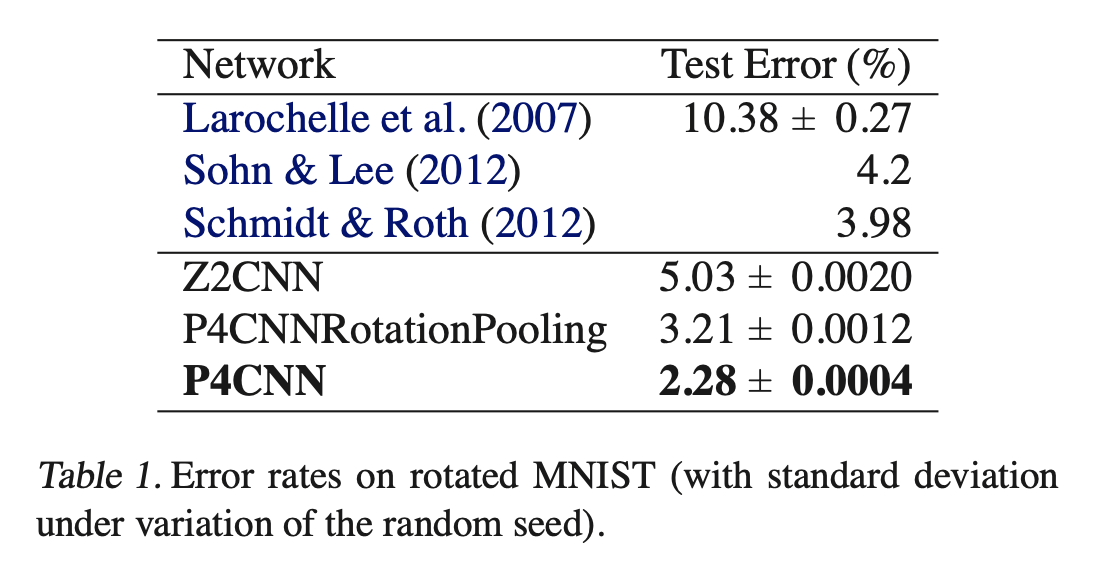
\includegraphics[width=\linewidth]{Screenshot 2024-01-13 at 11.28.16 AM.png} % replace with your first image file
        % \caption{Caption for image1}
    \end{minipage}%
    \begin{minipage}{0.5\textwidth}
        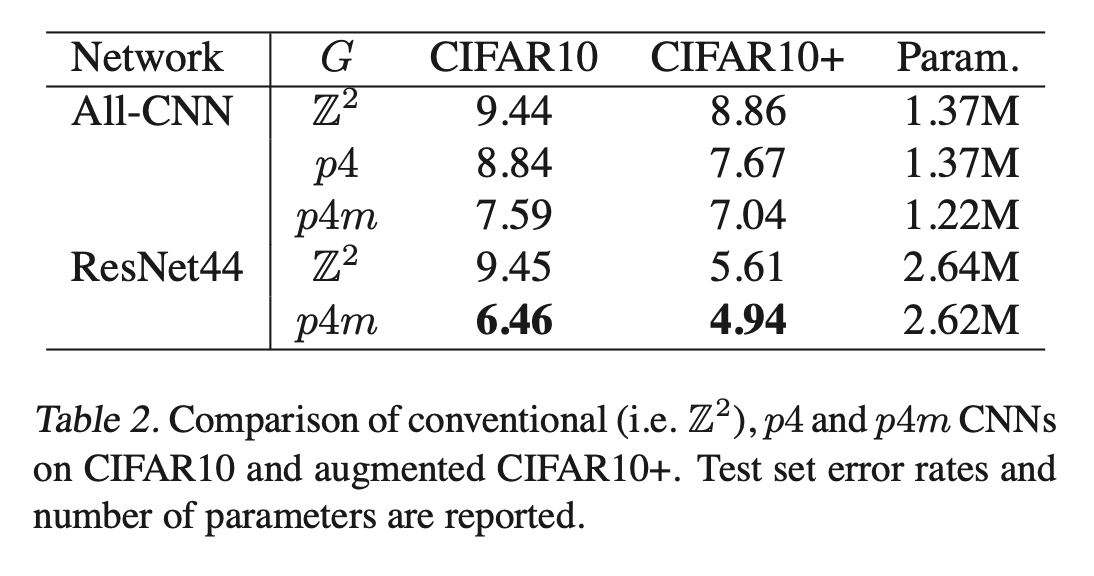
\includegraphics[width=\linewidth]{Screenshot 2024-01-13 at 11.28.27 AM.png} % replace with your second image file
        % \caption{Caption for image2}
    \end{minipage}
\end{frame}

% Demonstration of the code
\section{Demonstration of the Code}
\begin{frame}{Implementation}
    \href{run:jupyter-notebook Users/danielralston/Desktop/ece594n/hw_papers/Cohen-Group_Equivariant_Convolutional_Networks-2016/main.ipynb}{Open main.ipynb}
\end{frame}

% Conclusion
\section{Conclusion}
\begin{frame}{Conclusion}
    \begin{itemize}
        \item $p4$ and $p4m$ convolution layers act as effective replacements for traditional convolutions, consistently improving network performance.
        \item Future work includes extending $G$-CNNs to hexagonal lattices and 3D space groups, expanding symmetries and potentially improving pattern recognition capabilities.
        \item Challenges remain in extending the method to continuous groups and managing the computational load for large transformation groups.
        \item This work exemplifies the "structured representations” philosophy, suggesting that adding mathematical structure to neural network representations could reveal deeper similarities between concepts.
      \end{itemize}
\end{frame}

% References
\begin{frame}{References}
    \begin{itemize}
        \item Taco S. Cohen and Max Welling. \textit{Group Equivariant Convolutional Networks}, 2016, arXiv:1602.07576 [cs.LG].
        \item Erik Bekkers. \textit{Group Equivariant Deep Learning (UvA - 2022)}. YouTube, Mar 26, 2022, \url{https://www.youtube.com/watch?v=z2OEyUgSH2c}.
    \end{itemize}
\end{frame}


\end{document}